\section{Anforderungsanalyse}


\subsection{VJing}

Die Pr\"asentation von visuellem Material setzt gewisse Technik vorraus, welches verschiedene Medienformate unterst\"utzt,
andere nur unter Umst\"anden und manches vielleicht gar nicht. Beispielsweise unterst\"utzt ein Videorecorder keine digitalen
Videodateien. M\"ochte man die Performance mithilfe von Videoclips realisieren und braucht Funktionen wie Zeitraffer oder
automatisches Vorw\"arts-R\"uckw\"arts-Abspielen ist eine Software gesucht die das kann. Legt man viele Videos \"ubereinander
setzt das gewisse Rechenressourcen vorraus, mit denen das Resultat dargestellt wird.

Vor allem auf der Softwareseite sind viele Abh\"angigkeiten zu beachten. Da bei dem VRC-Konzept das Abspielen von Videoclips
nicht verloren gehen soll, die Darstellung und Animation von 3D-Inhalten zu Musik prim\"ares Ziel sind, stellt sich die Frage
mit welche Libraries in Frage kommen.

Der Bedienbarkeit kommt auch ein eigenes Feld zu. Viele VJs benutzen MIDI Controller, um die Darstellung zu steuern, da
Potentiometer gef\"uhlvolles Einstellen von Parametern erm\"oglicht. Gleichzeitig muss ein VJ auf drastische \"Anderungen
an der Darstellung vorbereitet sein.

\subsubsection{Hardware und Software}

Die Hardware sollte mobil sein. Ein Videoprojektor und ein Laptop sind die Grundlage f\"ur das Performen. F\"ur die
Soundanalyse kann man direkt das Signal von einem Verst\"arker abgreifen oder \"uber ein Mikrofon aufnehmen. Gleichzeitiges
Abspielen von mehreren Visuals auf einmal sollte m\"oglich sein. Das Anordnen der Visuals in einem dreidimensionalen
Raum erfordert Software, die das kann und auf Hardwareseite ist 3D-Beschleunigung n\"otig.
\\
Ein Laptop, der mehrere Videoclips und 3D-Modelle auf einmal berechnet und dazu den Sound analysiert und mit der Szenerie
verkn\"upft um Animationen und Visualit\"at zu erzeugen, braucht ein gewisses Mass an Rechenkraft. Da nicht nur die
Grafikkarte zum Rendern beansprucht wird, sondern vor allem auch die CPU f\"ur das schnelle Analysieren des Sounds und
Ausf\"uhren von Funktionen zust\"andig ist, darf hier nicht gespaart werden. Je nach dem wie Aufw\"andig die Szenerie
gestaltet ist ergeben sich Mengen von Polygonen, die transformiert werden m\"ussen. Auch hier sollten gen\"ugend
Leistungsreserven vorhanden sein, weshalb von Integrierten Grafikkarten abzuraten ist, da dedizierte Grafikkarten
momentan mehr Leistung haben.

Laptops, die f\"ur Computerspiele, technisches Zeichnen, Bilder- und Videoverarbeitung  konstruiert sind
verf\"ugen meist schon \"uber eine dedizierte Grafikkarte und eine besserer CPU als regul\"arer B\"urorechner.
\\
Hinsichtlich Kosten und Plattformwahl soll m\"oglichst freie Software verwendet werden. Eine leicht erlernbare
Programmiersprache zur Erstellung von Visuals soll es VJs mit mit geringen Programmierkenntnissen erm\"oglichen Visuals
f\"ur das Pr\"asentationsprogramm zu programmieren. Eine freie Grafikbibliothek wie OpenGL bietet eine Grundlage f\"ur
Rendering der Szenerie, jedoch stellt das Programmieren von OpenGL eine gro\ss e H\"urde f\"ur VJs mit nicht so tiefen
Programmierkenntnissen dar. Deher muss es die Komplexit\"at von OpenGL vereinfacht werden und Bibliotheken die auf OpenGL
aufsetzen benutzt werden.


\subsubsection{Bedienbarkeit}

F\"ur die Bedienung sollen standard Eingabeger\"ate wie Tastatur und Maus gen\"ugen. Vor allem die Einstellung der Ansicht
und Positionierung der Visuals in einem 3D-Raum muss auf einer Tastatur komfortabel m\"oglich sein - und das
wom\"oglich stundenlang. \"Uberblendungen und Visualwechsel beinhalten viele Aktionen wie das \"Andern von Transparenzen oder
Farben und muss fl\"ussig machbar sein. Die Ansicht durch eine virtuelle Kamera erfordert eine bewegliche Kamera. Bei
Rotationen der Kamera ist es wichtig die Orientierung nicht zu verlieren.

Eine Kombination aus Spielsteuerung f\"ur das ansteuern der Visual-Objekte und der Kamera scheint mit einer Tastatur
realisierbar und sinnvoll. Das Anzeigen und Einstellen von Statusinformationen von Kamera,
Soundanalyse und aktiven Visuals sowie die \"Ubersicht der verf\"ugbaren Visuals erfordert eine geeignete
Benutzerschnittstelle mit Panelen an denen Parameter abgelesen und ge\"andert werden k\"onnen.

Wichtig ist eine Reservierung von Tasten auf der Tastatur  f\"ur die Steuerung der ins Visual individuell einprogrammierten
Routinen.


\subsection{Visuals}

In dem VJ-Konzept ist der Fokus auf eine liberale Visualgestaltung ausgerichtet. Operationen wie Verschieben, Skalieren,
Rotieren und transformation zu Musik sollen jedem Visual aufgrund seines Charakters als Objekt in einem 3D-Raum m\"oglich sein.
Der Sound
soll von Visuals genutzt werden k\"onnen um Effekte auszul\"osen oder zu beeinflussen. Visuals bestehen bspw aus Punkten die zu
geometrischen Formen verbunden werden k\"onnen. Vorgefertigte 3D-Modelle sollen unterst\"utzt werden. Texturen k\"onnen
aus Bilddateien, Shaderprogrammen oder Videoclips bestehen. Durch das Programmieren der Visuals hat man
die M\"oglichkeit eigene Bibliotheken zu benutzen und Algorithmen zur Visualisierung zu implementieren.

\subsubsection{Erstellen}

F\"ur das Erstellen von Visuals ist es wichtig, dass der K\"unstler seine Visualidee verwirklichen kann. G\"angige
Formate f\"ur Bilddateien und Videos m\"ussen unterst\"utzt werden. Dadurch hat der (VJ)K\"unstler die M\"oglichkeit
verschiedene Tools zu benutzen um Bilder oder Videos zu pr\"aparieren. Im 3D-Raum k\"onnen diese dann als Texturen auf
Fl\"achen dargestellt werden.

Vor allem soll aber der VJ auch Punkte zu Poligonnetzen verbinden k\"onnen. So k\"onnen 3D-Modelle mit 3D-Grafikprogrammen
wie bspw Blender erstellt und in Visuals verwendet werden. Dadurch ist es auch m\"oglich vorgefertigte 3D-Modelle aus dem
Internet zu benutzen, welche von Anbietern zum Beispiel f\"ur CAD (Computer Aided Design), oder Spiele zum Download bereitgestellt
werden. Manche Formate bieten die M\"oglichkeit Animationen zu direkt im Model zu definieren. Unabh\"angig von Formaten
m\"ussen die Inhalte auch durch selbstgeschriebene Funktionen animierbar sein.

Mit eigens definierten Funktionen kann man auf die Skalierung, Farbe, Transparenz oder Positionierung Einfluss nehmen.
Das Soundsignal als wichtiger Bestandteil muss in Funktionen verarbeitbar sein. Durch die Analyse des Soundsignals k\"onnen
sich Funktionen dynamisch gegenseitig aufrufen und mit der k\"unstlerischen Intention verkn\"upft werden. So kann das
Visual programmiert werden auf B\"asse vorprogrammierte Effekte auszul\"osen.

Mit der Programmierung der Tasteneingabe kann das Visual gesteuert werden. Die Zustandsa\"nderung auf eine Tasteneingabe
muss bei der Erstellung definiert werden k\"onnen. Auch hierbei sind Funktionen die Grundlage daf\"ur.

primitive, 3d meshes,
fertige modelle mit blender
videoclips
tastenbelegung


\subsection{Darstellung}

Ein Programm zur Darstellung der Visuals ist n\"otig um alle Visuals mit dem Soundsignal zu versorgen, Eingaben entgegen
nimmt und auf Parameter der Visuals zugreiffen kann.


Das Programm stellt den 3D-Raum bereit in denen die Visuals geladen werden k\"onnen sowie eine \"Ubersicht \"uber
Parameter, Eingaben und Metainformationen \"uber die Zust\"ande der Visuals. Eine \"Ubersicht \"uber die Positionen
der Visuals und Kameras sowie der Ausrichtung der Kamera hilft dabei Szenen und Kameraeinstellungen zu koordinieren.

Diese Anforderungen k\"onnen in einer GUI untergebracht werden. Eine GUI fasst dabei Eingabeschnittstellen f\"ur die Visuals,
die Kameras und Soundeinstellungen zusammen, an denen die wichtige Daten \"uber den Zustand des Dargestellten abgelesen
werden k\"onnen.

Eine Ansicht durch eine Kamera wird dabei in Vollbildschirmmodus an das Ausgabeger\"at (Videoprojektor) geschickt. Eine
andere Ansicht in den Raum erm\"oglicht das direkte Interagieren mit Visuals und Kamera. Diese Ansicht soll den
Computerspielcharakter bereitstellten wodurch direkte Manipulation an Rotation und Position m\"oglich ist.

%Dabei m\"ussen verschiedene Tasks ausgef\"uhrt werden.
%programm zur das sound verarbeitet,
%parameter einstellung
%taskmanager,
%Eingabe verarbeiten

%\subsubsection{3D Raum und Camera}

%Durch die Ansicht des 3D-Raums durch die virtuelle Kamera wird der 3D-Raum zum Beh\"alter f\"ur Visuals, der betrachtet wird.
%Die Positionierung der Kamera und der Visuals

%container fuer visuals
%beinhaltet cameras zur ansicht
%Camerapositionierung

\subsubsection{Performen}

Die Performance des VJs besteht aus dem Laden und Entfernen von Visuals in dem 3D-Raum. Visuals werden um die
Kamera angeordnet und bilden die Szenerie. Bei \"Anderungen in der Musik wird die Szenerie angepasst oder der
Blickwinkel auf die Szenerie ge\"andert.

Musik enth\"alt oft H\"ohepunkte und viele k\"unstlerische Stilmittel.
Anhand der akustischen Wahrnehmung des VJs kann an Wendepunten in der Musik in Echtzeit die Performance des VJs
an die Musik anpasst werden. Durch hineinfaden eines anderen Visuals, einem Schnitt oder dem Ausl\"osen eines
Effekts erh\"alt die Musik ihre visuelle Individualit\"at w\"ahrend des Events.

Dabei soll das Programm Operationen wie Schnitte, Kamerafahrten, Positionierung und Rotationen, Fading oder
\"Anderungen an der Kameraeinstellung schnell auf Visual und Kamera f\"ur den VJ schell ausf\"uhrbar gestalten.
Hauptaugenmerk f\"ur das Performen ist die Usability. Da die Eingabeger\"ate f\"ur den Anfang aus
Maus und Tastatur bestehen muss ein geeignetes Bedienkonzept erarbeitet werden.

\section{Entwurf}

Beim Entwurf m\"ussen \"Uberlegungen getroffen werden, welche die Auswahl der Software im Vorfeld auf
die in Frage kommenden Plattformen und n\"otige Programmbibliotheken reduziert. F\"ur die Implementierunge
wichtige Datenstrukturen m\"ussen so gew\"ahlt sein, dass man zur Laufzeit den Variablenzustand von Sound-
und Bedienungseingabe geschickt an allen relevanten Stellen abrufen und \"andern kann.

\begin{figure}[h!]
    \centering
    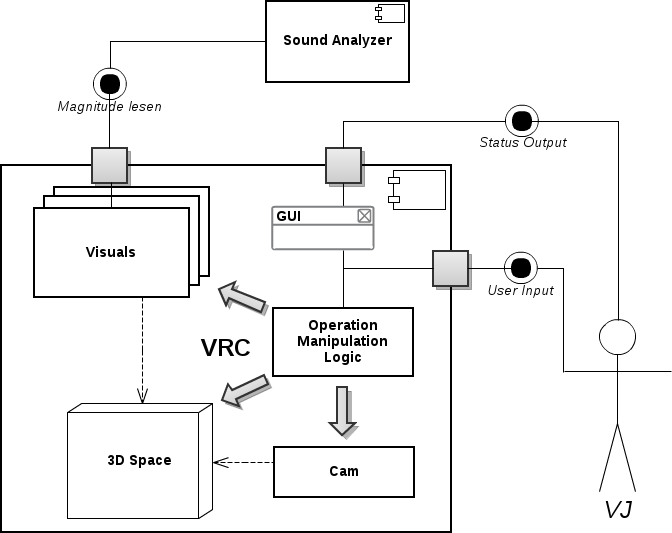
\includegraphics[width=1\textwidth]{pictures/vrc-component1.png}
    \caption{Strukturdarstellung des VJ-Konzeptprogramms VRC, bestehend aus Soundeingabe und einem Container f\"ur
    3D-Raum und Visuals welche von einem User f\"ur die VJ-Performance genutzt werden.}
\end{figure}

Das Konzept weist eine grundlegende Struktur aus 3D-Raum, Visuals, Soundeanalyse und Bedienkonzept auf


\subsection{\"Uberlegungen}

OpenGL entwickelte sich zum Industriestandard f\"ur interaktive 2D und 3D-Grafiken (* http://www.opengl.org/about/ )
und bietet eine umfangreiche Programmierschnittstelle f\"ur Grafikprogrammierung. Diese Schnittstelle wird durch
Grafikkarten hardwareseitig unterst\"utzt. F\"ur die meisten popul\"aren Sprachen gibt es Sprachanbindungen mit denen
man auf die Schnittstelle direkt zugreiffen kann.

Spiel-Engines als Programmierger\"ust erscheinen vorteilhaft um 3D-Grafiken in Szene zu setzen. Durch die Beschr\"ankung
auf standard Eingabeget\"ate sind Spiel-Engines hervorragend f\"ur die Verarbeitung von Benutzereingabe und Steuerung
des 3D-Raums geeignet. Auch das Erstellen von Visuals erf\"ahrt durch die Verwendung von Spiel-Engines Vorteile. Elemente
werden in Visuals gruppiert und mit Funktionen unter Einbezug verschiedener Parameter modifiziert/transformiert. Anhand
des Soundsignals k\"onnen ausgew\"ahlte Parameter dem musikalischen Zufall \"uberlassen werden. Dadurch wird eine
akustisch-visuelle Koppelung zwischen Visual und Umgebung m\"oglich. Die Soundeingabe soll m\"oglichst unabh\"angig von
technischen Faktoren m\"oglich sein. Laptops haben meist schon standardm\"a\ss{}ig ein Mikrofon eingebaut, das man als
standard Eingabeger\"at bei Performances nutzen kann.

Wichtig vor allem ist, dass man Effekte durch Tastendruck ausl\"osen kann. Dazu m\"ussen Visuals frei programmierbar sein
um mit Code den Ablauf des Effekts zu definieren. Dadurch dass Tasten mit Programmierung belegt werden k\"onnen, sind f\"ur
die Visuals individuelle Funktionen programmierbar. Durch Anwendung der objektorientierten Programmierung k\"onnen
Funktionen (Methoden) k\"onnen Objekte als Container f\"ur Funktionen und Daten dienen. Objektorientiertes Programmieren
eignet sich also f\"ur Visuals.


%OpenGL - Hardwarebeschleunigt
%Framework f\"ur OpenGL - Game Engine, SDL, Processing
%Mikrofon als Soundinput - standard laptops haben bereits mic
%Python/C++/Java - Comparision Libraries/Bindings
%Libraries - Soundanalyse, GUI,
%Datenstrukturen f\"ur Visuals
%Visualrealisierung - OpenGL, eigene Funktionen

\subsubsection{Datenstrukturen}

Um die Visuals im Programm vorzuhalten und kann eine Liste mit Verweisen auf die Visuals verwendet werden. F\"ur
die Visual-Elemente muss der 3D-Raum eine Datenstruktur vorhalten in den die Elemente hineingeladen werden k\"onnen.
Daf\"ur eignet sich eine Baumstruktur ganz gut. Der 3D-Raum stellt die Wurzel des Baums dar, jedes Visual ist ein
Kind des 3D-Raums. Ein Visual besteht aus einem Knoten, der als Wurzel f\"ur die Visual-Elemente fungiert
(siehe Abbildung). Dieser Baum stellt den Szenengraphen dar, in dem die OpenGL-Objekte der Visuals, wie Modelle, Texturen
oder Videos geladen werden.

\begin{figure}[h!]
    \centering
    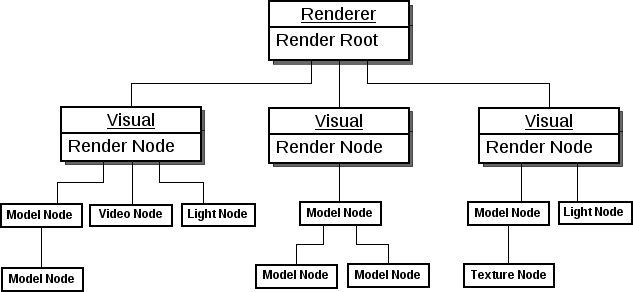
\includegraphics[width=1\textwidth]{pictures/data_structure1.png}
    \caption{Skizze eines Szenengraphen}
\end{figure}

%Liste mit VisualObjekt-Referenzen
%Visual-Elemente werden von Visuals in Graphen geladen
%VisualObjekt haelt Referenzen auf seine eigenen Elementobjekte im Graph der VisualElemente
%3D-Raum wird aufgebaut anhand des Graphen, der den zu sehenden Inhalt enth\"alt

\subsubsection{Soundanalyse}

Es gibt verschiedene M\"oglichkeiten Sound zu analysieren. Bei diesem Entwurf wird Wert darauf gelegt, dass
Soundwerte auf einfache Art in den Visuals verarbeitet werden k\"onnen. Es sollen B\"asse, Mitten und H\"ohen
als Werte von  0 bis X abgelegt werden.

Die Soundanalysekomponente muss kontinuierlich die Soundeingabe verarbeiten. Das aufgenommene Frequenzband
wird unterteilt in Bassband, Mittelband und H\"ohenband.
Das Bassband erstreckt sich \"uber die Frequenzen 0Hz bis 100Hz, die Mittelt\"one \"uber 100Hz bis 1000Hz,
und die Hoehen \"uber 1000Hz bis 44100Hz.
F\"ur jedes Band wird eine Magnitude berechnet, welche die Intensit\"at Samples auf den drei B\"andern angibt.
Dem Mikrofonsignal werden kontinuierlich Samples entnommen um die Magnitude \"uber den Frequenzb\"andern zu
messen und in Soundzustandsvariablen zu speichern. Das Soundsignalsample ist ein Vektor aus 16Bit Integer-Werten -
f\"ur jede Frequenz ein Integer.

Eine einfache Methode den die Musik zu analysieren und einen Beat zu erkennen ist beispielsweise das Vergleichen
der Magnitude mit einem Grenzwert. Liegt die Magnitude \"uber dem Grenzwert, so kann das als Beat interpretiert
werden worauf eine Aktion folgen kann.

\subsubsection{Bedienung}

Da in den Anforderungen, die Benutzung von standard Eingabeger\"aten gefordert ist stellt vor allem die
Tastatur zur Steuerung von Visuals eine gute Plattform dar. Das Virtual Room Concept verh\"alt sich von der
Navigieren im 3D-Raum \"ahnlich dem des Bewegens von Aktoren in Computerspielen oder Arbeiten mit 3D-Programmen
wie Blender. In Computerspielen ist das was der Spieler sieht eine Ansicht einer virtuellen Kamera auf die ihn
virtuell umgebende Szenerie. Eine Grundlage zum Spielen ist das Bewegen des Agenten im Spiellevel, was dem
Bewegen einer virtuellen Kamera in einem 3D-Raum entspricht.

Viele Spiele, allen voran First-Person-Spiele (FPS) haben oft f\"ur das Bewegen des virtuellen Agenten standardm\"a\ss{}ig
die selbe Tastenbelegung. Auch andere Funktionen wie die Auswahl von Gegenst\"anden ist oft \"ahnlich belegt.
Der gr\"o\ss{}te Unterschied zu den meisten FPS ist es wohl, dass man die Kamera, bzw die Visuals zus\"atzlich um die
L\"angsachse rotieren moechte.

In diesem Entwurf wird die Bedienung von FPS f\"ur die Kamera und Visuals adaptiert. F\"ur die Rotationen wird
auch die Tastatur verwendet. Hierf\"ur werden zus\"atzlich Belegungen definiert. Diese unterscheiden sich von
denen in FPS. In FPS wird f\"ur die den Nick- und Gier-Winkel h\"aufig die Maus verwendet. Da f\"ur Kamera und
Visual jeweils Rotationen und Bewegungen m\"oglich sein sollen, wird die Bedienung f\"ur diese Aktionen
vereinfacht indem die selbe Belegung f\"ur Visual und Kamera gilt.

Die Abbildung zeigt den Entwurf f\"ur eine m\"ogliche Tastenbelegung.

\begin{figure}[h!]
    \centering
    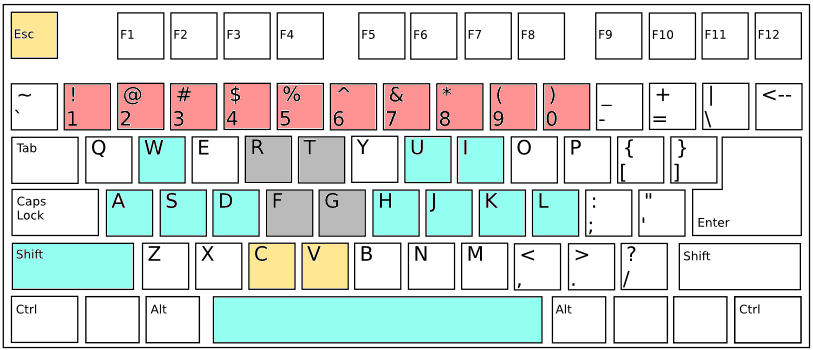
\includegraphics[width=1\textwidth]{pictures/usage_keyboard_layout1.png}
    \caption{Skizze eines Szenengraphen}
\end{figure}

F\"ur das Navigieren in der grafischen Oberfl\"ache wird die Maus verwendet.

%Tastatur, Maus
%Belegung Feste und programmierbare
%Bild

\subsubsection{Grafischen Oberfl\"ache}

In der grafischen Oberfl\"ache werden Daten aus dem Zustand des VRC aufbereitet, um Statusinformationen \"uber die
Visuals und Kamera anzuzeigen. Ausserdem werden \"uber die grafische Oberfl\"ache die Visuals in den 3D-Raum hinzugef\"ugt
oder entfernt. Wichtige gemeinsame Funktionen der Visuals k\"onnen in der grafische Oberfl\"ache zusammengefasst und
der Manipulation zug\"anglich gemacht werden.

Es m\"ussen die wichtigen Entit\"aten zum VJing schnell abrufbar sein. Gleichzeitig hat man aber nur begrenzten Platz auf
dem Bildschirm um Vorschaufenster und Menus unterzubringen.
Durch eine geschickte Unterbringung der Entit\"aten in Menus die mit Reitern navigierbar gestaltet sind, kann man Menuelemente
f\"ur den Visualpool, geladene Visuals, Kamera- und Soundeinstellungen gruppieren.
%Eine geschickte Unterbringung der Entit\"aten unter Reitern
%kann man seperat Visualpool, geladene Visuals, Kamera- und Soundeinstellungen erm\"oglicht das Gruppieren der verschiedenen
%Oberfl\"achenelemente.
Die verschiedenen Entit\"aten Sound, Visuals und Kamera haben auch ihre eigenen Anforderungen an
Schnittstellen. So haben Visuals eine Schnittstelle f\"ur Skalierung, Transparenz, die Kamera aber nicht. Da es sich um
eine \"uberschaubare Menge an Entit\"aten handelt ist ein Reiterlayout f\"ur den VJ beim VJing ausreichend um Kontrolle
\"uber die Visualwerte zu behalten.

\begin{figure}[h!]
    \centering
    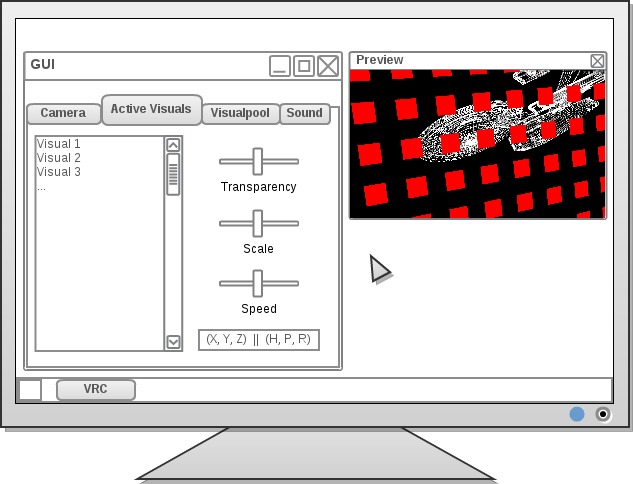
\includegraphics[width=1\textwidth]{pictures/gui1.png}
    \caption{Skizze der Grafischen Oberfl\"ache auf einem Monitor als Fenster f\"ur das Virtual Room Concept und die Vorschau}
\end{figure}

Das Resultat, welches auf im Vorschaufenster zu sehen ist wird auf \"uber einen zweiten Videoausgang ohne Fensterrahmen auf
einem externen Ausgabeger\"at angezeigt.


\subsubsection{Engine}

Letztendlich braucht man ein Framework, mit dem die Grafikausgabe programmiert werden kann. F\"r die verschiedenen anfallenden
Aufgaben braucht man einen Taskmanager, der wiederholende Aufgaben erledigt. Das Framework dient als Schicht zwischen OpenGL
und den zus\"atzlichen Komponenten wie Soundanalysierer und grafischer Oberfl\"ache.

Spiel-Engines besitzen Eigenschaften, die f\"ur sie Realisierung der Virtual-Room-Concept-Programms essentiell sind. Vor
allem bieten sie eine Datenstruktur zur Unterbringung der 3D-Geometrie - meist einen Szenengraphen in Baumstruktur.
Auf den Szenengraphen wird \"uber eine Schnittstelle in der Spiel-Engine zugegriffen. Ein Task-Manager der kontinuierlich
die Benutzereingaben und die Soundanalyse verwaltet erleichtert das Programmieren der Ablauflogik innerhalb des VRC-Programms.
Zum einen mussen die Visuals stets mit Soundwerten versorgt werden, zum Anderen m\"ussen die Eingaben des Benutzers
entgegengenommen und ausgef\"uhrt werden.

F\"ur die Visualprogrammierung ist die Wahl einer Spiele-Engine vorteilhaft, da man eine Abstraktionsebene f\"ur das
Zusammenstellen von Geometrie und 3D-Modellen in den Szenengraphen hat.
%Beim Performen der Visuals ist es wichtig die Visuals in die Szenerie laden und entfernen zu k\"onnen.
Auch f\"ur das Performen eignen sich Spiele-Engines gut und besitzen dank des
Szenengraphen und seinen Schnittstellen eine einfache M\"oglichkeit Visuals zu laden und zu entfernen. Die Betrachtung
der Szenerie durch eine virtuelle Kamera ist eine grundlegende Anforderung f\"ur Spiel-Engines, sowie f\"ur das
VRC-Programm.

Das Angebot an freien Spiel-Engines ist relativ gro\ss{}, jedoch sollte die Spiel-Engine so gew\"ahlt werden, dass sie
sich gut mit den anderen  Komponenten des VRC-Programms und ihren Bibliotheken verwenden l\"asst.

Neben vielen C++ und Java Spiel-Engines existieren auch f\"ur viele andere Sprachen Spiel-Engines. Dabei ist entscheidend,
dass die Spiel-Engine einen gro\ss{}en Benutzerkreis haben damit ein Interesse besteht, die Spiel-Engine auch in Zukunft
aktualisiert und weiterentwickelt werden.

Python erfreut sich in der 3D-Gestaltung einer hohen Popularit\"at. Programme wie Blender und auch Modul8 besitzen eine
Python-Sprachanbindung. Blender verf\"ugt sogar \"uber eine eigene Spiel-Engine in Python. Mit Python als Sprache f\"ur
eine Spiel-Engine erleichtert man durch die relativ einfache Syntax VJs den Einstieg in das Konzept. Eine gute Dokumentation
der Sprache und der Spiel-Engine hilft bei der Erstellung der Prototyps und der Visuals enorm. Anhand dieser Aspekte
l\"asst sich die Wahl einengen in eine OpenGL-basierte Spiel-Engine f\"r Python. Die bekanntesten Vertreter von
Spiel-Engines f\"ur Python sind Python-Ogre, Spring, Blender oder Panda3d.

Weitere Vorteile von Spiel-Engines sind
\begin{itemize}
    \item Konvertierungswerkzeuge f\"ur viele 3D-Modellingtools
    \item Shader-Generatoren f\"ur Spezialeffekte
    \item Kollisionsdetektion und Unterst\"utzung eines Physik-Systems
\end{itemize}

%Panda3d
%3d-Raum
%Kamera (eigene subsubsection)

%\subsubsection{Szenengraph}
%Renderer

\subsubsection{Visual-Klasse}

Visuals besitzen durch ihre Anforderungen an Beweglichkeit, Skalierung und andere gew\"unschte Manipulationsm\"oglichkeiten
eine Menge an gleichen Funktionen, welche diese Operationen umfassen. Da Visuals als Objekte gedacht sind l\"asst sich deren
Charakterisierung von einer Klasse ableiten.

\begin{wrapfigure}{r}{0.5\textwidth}
    \begin{center}
        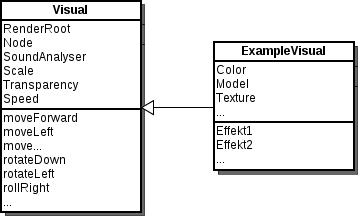
\includegraphics[width=0.48\textwidth]{pictures/visualclass1.png}
    \end{center}
    \caption{Visual-Klasse vererbt einem Visual-Objekt die n\"otigen Daten und Funktionen um im Programm an Soundanalyse
        und Szenengraph angebunden und einheitlich beweglich zu sein.}
\end{wrapfigure}

Durch die richtige Initialisierung und einer Standardeinstellung ist das \"Uberschreiben und Erweitern der Visual-Klasse im
Objekt m\"oglich.
Die Visual-Klasse besitzt einen Konstruktor mit dem die Initialisierung f\"ur das VRC-Programm vorgenommen wird. So wird
der Knoten, an den alle weiteren 3D-Elemente gekn\"upft werden erstellt, Referenzen auf andere Komponenten des
VRC-Programms werden angelegt.
Weiter werden Funktionen f\"ur die Bewegung und Rotation der Visuals schon in der Visual-Klasse definiert. Mit diesen
Funktionenen ist es m\"oglich die Visuals im 3D-Raum anzuordnen.

Diese Eigenschaften k\"onnen von Visuals geerbt werden und stehen ihnen dann zur Verf\"ugung. Mit der Verwendung einer
Visual-Klasser erreicht man, dass sich Visuals trotz individueller Programmierung einheitlich in das VRC-Programm
einf\"ugen und steuern lassen.

\section{Prototyp}

\subsection{Softwarewahl}

Nach erfolglosen Versuchen mit Processing einen Prototypen zu erstellen begann die Suche nach Alternativen. Erst
wurden noch javabasierte Bibliotheken f\"ur OpenGL ausprobiert. Nachdem aber schnell klar wurde, dass keine der
getesteten Bibliotheken in der Lage war simpel und komfortabel zwei Fenster mit dem selben Inhalt darzustellen begann
die fiel der Fokus auf Spiel-Engines. Wichtig wurde immer mehr, dass eine gute Dokumentation und eine gut aufgestellte
freie Entwicklergemeinschaft wichtig sind f\"ur den Erfolg des Projekts. Durch eine gute Dokumentation ist es
leichter die verwendete Software zu erlernen, dank einer aktiven Benutzer- und Entwicklergemeinschaft werden spezifische
Fragen in Internet-Foren oder Chat-R\"aumen schnell beantwortet.

Letzendlich fiel die Wahl der Game-Engine auf Panda3d. Mit Panda3d wurden zu Beginn Testprogramme erstellt, mit denen
die Anforderungen an Funktionalit\"at ausgetestet werden. So wurde erst einmal versucht die Ausgabe des Programms
auf einem undekorierten Fenster auf ein Ausgabeger\"at in Form von Videoprojektor auszugeben. Als diese Funktionalit\"at
durch kleine Testprogramme erreicht worden ist, ging es darum zu sehen, wie sich die Ansicht auf die 3D-Szenerie
bedienen l\"asst. Dazu wurde ein kleines Programm mit ein paar geladenen Models geschrieben und eine Kamera hineingesetzt.
Nachdem erfolgreich die Kamerabedienung programmiert worden ist, waren das die Kriterien f\"ur die Entscheidung bei der
verwendeten Spiel-Engine zu verbleiben und darauf aufzubauen. Wichtig bei der Wahl der Spiel-Engine war auch, dass
sie nicht veraltet ist und Techniken wie Shaderprogrammierung, Schatten und Licht in verschiedenen Variationen besitzt und
eine klare Programmierkonvention hat. Panda3d erf\"ullt all diese Eigenschaften und noch viele Mehr wie Physik-Engine und
Shader-Unterst\"utzung.

F\"ur die Soundanalyse-Komponente ist wichtig, ohne gro\ss{}e Schwierigkeiten die Hardware anzusprechen und den Sound
dar\"uber auszulesen. Bei der Berechnung der Magnituden muss man \"uber ein Vektor aus 16Bit nat\"urliche Zahlen iterieren.
Dabei muss man die Laufzeit beachten. Es gibt Bibliotkeken f\"ur Python zum Auslesen des Signals \"uber Pulse-Code-Modulation.
Einen Algorithmus zur Berechnung der Magnitude auf den Frequenzb\"andern der tiefen, mittlere und hohen T\"one konnte
aus einem C++-Programm \"ubersetzt, welches eine \"anliche Soundanalyse-Komponente verwendete (reference auf liveGL von phreax)

Panda3d bietet die M\"oglichkeit verschiedene Wrapper f\"ur GUI-Toolkits zu verwenden, darunter wxPython (ref)  und TKinter (ref).
WxPython ist ein Wrapper f\"ur die wxWidgets-Klassenbibliothek (ref), TKinter ist eine Sprachanbindung an den Tk (ref).
Tkinter entwickelte sich zum quasi-standard GUI-Paket f\"ur Python und wird mit Python zusammen ausgeliefert.
Tkinter eignet sich zum schnellen Prototypenbau f\"ur grafische Oberfl\"achen. F\"ur den VRC-Prototypen wurde die
Tkinter-Bibliothek gew\"ahlt.

\subsection{Datenstrukturen}

Innerhalb der Testprogramme wurden Datenstrukturen f\"ur die Bedienung und das Handhaben der Visuals verwendet.
Dabei erwies sich assoziatives Datenfeld als geeignet, um die Tastatureingabe entgegenzunehmen und f\"ur ein
Bedienschl\"usselwort zu speichern. Panda3d verarbeitet Tastendruck- und Tastenfreigabe-Events. Die Tastenzust\"ande
lassen sich bin\"ar als 1 und 0 darstellen, wobei 1 gedr\"uckt repr\"asentiert und 0 nicht gedr\"uckt bedeutet.
Um nun f\"ur eine Operation den Zustand zu speichern wird die Tastatur zyklisch abgefragt. Wenn eine Taste gedr\"uckt wird
und einer Operation entspricht so wird der Wert dieser Operation auf 1 gesetzt, wie anhand des Codebeispiels gezeigt.

\begin{lstlisting}

if key == "a": setOperationMap('move-forward', 1)
if key == "a-up": setOperationMap('move-forward', 0)

\end{lstlisting}

So wird der Zustand der Eingabe an einer Stelle im Speicher vorgehalten und ist in anderen Teilen des
Prototypen leicht abrufbar.

In einer Listen werden die Verweise auf geladene Visuals vorgehalten. Dadurch k\"onnen Funktionen leicht auf allen
geladenen Visual-Objekten ausgef\"uhrt werden, wie beispielsweise das Versorgen mit den Sound-Messwerten.

Der Szenengraph ist eine baumartige Datenstruktur. Panda3d besitzt Schnittstellen um Knoten und deren Unterknoten
aus dem Baum zu entfernen und an einer anderen Stelle im Szenengraphen anzuh\"angen. So k\"onnen Visuals, die nicht mehr
performt werden sollen aus dem Graph entfernt werden wodurch Rechenressourcen frei werden.

\subsection{Software-Architektur}

Das Zusammenf\"uhren von Visuals, Sound-Messwerten und GUI erfordert eine durchdachte Architektur f\"ur das VRC-Programm.
Die erforderlichen Komponenten lassen sich zu Klassen zusammenfassen. Das Klassendiagramm (siehe Abb X) zeigt die
Assoziationen der Klassenobjekte untereinander.

\begin{figure}[h!]
    \centering
    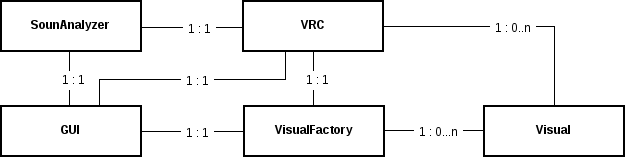
\includegraphics[width=1\textwidth]{pictures/classdiagram1.png}
    \caption{grobes Klassendiagramm mit Assoziationen}
\end{figure}

\subsubsection{VRC-Klasse}

Die VRC-Klasse erbt von der Spiel-Engine. So bekommt sie unter Anderem die Puffer f\"ur den 3D-Raum und den Taskmanager
vererbt, die die Grundlage f\"ur das Konzept bilden. Mithilfe des Taskmanagers kann man wiederkehrende Tasks wie
das Abfragen des SoundAnalyzers und des Tastaturzustands ausf\"uhren. Dadurch vermeidet man das Programmieren in einer
Hauptschleife.
In ihrem Konstruktor initialisiert die VRC-Klasse, die f\"ur sich ben\"otigten Objekte der anderen Klassen.
In Variablen und einer Liste f\"ur Visuals werden die Referenzen auf diese Objekte gespeichert.

Neben den f\"ur das Konzept wichtigen Objekte, wird in der VRC-Klasse auch die Initialisierung der Spiel-Engine
vorgenommen. Unter anderem werden Fenster erstellt, und die Kameras den Fenstern zugewiesen.

\begin{figure}
\begin{lstlisting}
props = WindowProperties()
props.setSize(size)
props.setUndecorated(True)
props.setOrigin(0,0)
self.otherWin = self.openWindow(props, makeCamera = 0)
self.win.setClearColor((0,0,0,1))
self.otherWin.setClearColor((0,0,0,1))
\end{lstlisting}
\end{figure}

Ausserdem wird in der VRC-Klasse der Bedienmechanismus implementiert. Der Bedienmechanismus schaltet zwischen
Visualmodus und Kameramodus zwischen Funktionen um, die f\"ur die Tastatureingabe in dem assoziativen Datenfeld
f\"ur Operationen richtig schalten. Daf\"ur wird mithilfe des Taskmanagers der Spiel-Engine der Tastaturzustand
kontinuierlich abgefragt und anhand dessen die Aktionen ausgef\"uhrt.
Die Spiel-Engine implementiert anhand von Event-Polling das Belegen
von Tasten mit Funktionen.
Da die VRC-Klasse von der Spiel-Engine erbt kann man ganz Einfach im Konstruktor die Belegung
der n\"otigen Tasten initialisieren und an Funktionen kn\"upfen.

\begin{lstlisting}
self.accept('a', self.setOperation, ['a'])
self.accept('a-up', self.setOperation, ['a-up'])
...
self.taskMgr.add(self.executeOperation, 'keyboardaction')
self.taskMgr.add(self.spreadTheBeat, 'sound')
\end{lstlisting}

In der executeOperation-Funktion wird anhand des Bedienmodus die entschieden ob die Kamera-Operationen oder
Visual-Operationen ausgef\"uhrt werden. Die spreadTheBeat-Funktion f\"uhrt auf allen Visuals eine Methode zum
Reagieren auf. Dadurch erhalten die Visuals gleichzeitig einen Art Tick, anhand Sie selbst kontinuierlich
Funktionen implementieren k\"onnen.

\subsubsection{SoundAnalyzer-Klasse}

In der Soundanalyzer-Klasse werden Bibliotheken f\"ur die Schnelle Fouriertransformation und f\"ur den Zugriff
auf das PCM-Signal verwendet um \"uber die drei Frequenzb\"ander B\"asse, Mittelt\"one und H\"ohen das Spektrum
zu analysieren und als Gleitkommazahl zu repr\"asentieren.



\subsubsection{Visual-Klasse}

Die Visual-Klasse stellt Methoden f\"ur das Bewegen und Rotieren der Visuals bereit. Sie wird mit einer Referenen
auf den SoundAnalyzer und auf den 3D-Raum initialisiert.
Es wird ein Platzhalter-Knoten f\"ur den Szenengraph angelegt, der Ausgangspfad f\"ur die anderen Elemente des Visuals ist.
Dieser Knoten wird in den Bewegungsmethoden verwendet um das Visual durch den Raum bewegen zu k\"onnen. Alle Elemente,
die an diesen Knoten angef\"ugt werden bewegen sich dann relativ zum Platzhalter-Knoten mit.

\begin{lstlisting}
def __init__(self, render, loader, snd):
    self.snd = snd
    self.loader = loader
    self.render = render
    self.path = self.render.attachNewNode('dummy')
    self.path.setPos(0,0,0)
    ...
    self.setup()

def moveRight(self):
    self.path.setX(self.path, +self.visualMovementSpeed)
\end{lstlisting}

Au\ss{}erdem werden noch initiale Zustandsvariablen f\"ur die Bewegungsgeschwindigkeit, Transparenz und Skalierung definiert.
Der Konstruktor ruft zum Abschluss noch eine weitere leere Setup-Funktion auf. Diese Funktion ist daf\"ur gedacht,
als Framework-Funktion in den von der Visual-Klasse abgeleiteten Visuals \"uberschrieben zu werden. Dadurch kann man
an diesem Punkt die visualspezifischen Elemente laden und einstellen.

Weiter wird eine Methode f\"ur das Entgegennehmen der Soundanalyse implementiert. Diese Methode ruft noch eine weitere
Platzhalter-Methode auf, die im eigentlichen Visual dann mit einem Algorithmus f\"ur das Reagieren auf den Sound
\"uberschrieben werden kann.

F\"ur die Effekte werden leere Methoden angelegt, die aus der VRC-Klasse durch die Bedienung ausgel\"ost werden. In den
einzelnen Visuals k\"onnen diese Methoden \"uberschrieben werden. Dadurch hat man ein Framework um sich f\"ur die
Tasten eigene Effekte anlegen zu k\"onnen.

\subsubsection{VisualFactory-Klasse}

Der Prototyp verwendet f\"ur das Initialisieren der Visuals eine Visual-Objektfabrik, da die Initialisierung eines Visuals
mehr als da Initialisieren des Konstruktor ben\"otigen kann. Dadurch hat man als Programmierer mehr Freiheiten aus dem
Visual-Framework auszubrechen und Ideen zu Realisieren, welche die Anbindung anderer Externer Bibliotheken oder Module
erfordern.
Der Konstruktor nimmt Referenzen auf 3D-Raum und SoundAnalyse-Objekt entgegen um damit die Visuals zu initialisieren.
Die Visual-Objekte werden unter einem Namen in einem W\"orterbuch angelegt.

\subsubsection{GUI}

In der GUI befinden sich Slider, Buttons und Listen mit denen die Einstellungen an Kamera, Visuals und SoundAnalyzer
vorgenommen werden k\"onnen. So wird \"uber die GUI mithilfe von Schiebern die Transparenz,
die Bewegungsgeschwindigkeit und Skalierung f\"ur die Visuals eingestellt. Mit einem Button k\"onnen die Visuals in den
Raum gesetzt und entfernt werden. Standardm\"a\ss{}ig werden die Visuals am Nullpunkt gesetzt. Die Namen der geladenen
Visuals erscheinen in einer Auswahlliste. Dort kann man ein Visual ausw\"ahlen, um es zu im Visualmodus bedienen.
F\"ur die Kamera kann die Sensitivit\"at \"uber einen Schieber eingestellt werden. Zur Soundanalyse koennen anhand von
drei Schiebern ein Grenzwert eingestellt werden, mit dem dann in den Visuals der aktuelle Messwert verglichen werden kann.
Dadurch kann man z.B. bei basslastigem Klang den Grenzwert erh\"ohen um die Reaktion der Visuals auf starke B\"asse zu
trimmen.

F\"ur den \"Uberblick sind Labels vorgesehen in denen die Positions- und Rotationsinformationen der Kamera und der Visuals
anzeigen. Au\ss{}erdem werden Informationen aus der dem Operationsw\"orterbuch angezeigt, wie bspw. ob die Kamera
im Vorschaufenster synchron mit der Kamera im Pr\"asentationsfenster ist, oder ob die Kamera auf ein Visual fixiert oder
frei ist.

\section{Usability Test}

Die Gebrauchstauglichkeit und Benutzbarkeit wird qualitativ anhand von vier Testpersonen ermittelt. Die Personen sollen
sich mit dem Programm vertraut machen, und die Bedienung ausprobieren. Danach wir den Testpersonen das VJing-Konzept
erkl\"art. Den Testpersonen werden Herangehensweisen f\"ur das Einfaden und Ausfaden der Visuals
gezeigt, um das Potential des Konzepts vorzustellen.

Nachdem die ersten Fragen der Testperson gekl\"art sind wird Musik abgespielt und das Programm neu gestartet. Die Testperson
muss von vorne starten ein Szenerie aufzubauen und eine Betrachtungsweise daf\"ur zu finden. Mittels Effekten und Transparenzen
wird versucht f\"ur ein bisschen visuelle Abwechslung zu Wendepunkten in der Musik zu sorgen.

Nachdem sich die Testperson mit \"Ubergangsmethoden und Effekten vertraut gemacht hat, und gelernt hat sich im 3D-Raum zu
orientieren, Visuals zu Positionieren und die Kamerabewegungen beherrscht, wird ein Szenario gestellt. Die Testperson soll
sich vorstellen auf einem Konzert zu drei Liedern Visuals performen. Dazu wird Hiphop und Elektronische Tanzmusik
verwendet. Bei Hiphop gibt es oft beim Refrain eine musikalische \"Anderung. Beispielsweise setzt ein zus\"atzliches
Instrument ein oder es wird in einer Pause kurz innegehalten und der Beat setzt wieder ein. Bei elektronischer
Tanzmusik sind Mittelt\"one, B\"asse und H\"ohen meistens gut voneinander unterscheidbar. Oft werden mit Tief- und
Hochpassfiltren gearbeitet um sogenannten Druck aufzubauen. Dabei wird die Musik mit Tiefpassfiltern ged\"ampft und wieder
aufgedreht. In solchen Momenten kann man irgend eine Aktion mit einem Visual oder mit der Kamera durchf\"uhren.

W\"ahrend des Test wurden die \"Au\ss{}erungen der Testpersonen in Stichw\"ortern notiert. Da die Testpersonen
unterschiedlichen Hintergrund haben, bringen sie unterschiedliche F\"ahigkeiten mit. Es testeten ein Fussballer ohne viel
Computerkenntnisse, eine Linguistikstudentin, die Programmiergrundlagen beherrscht,
ein Filmemacher der Dozent f\"ur neue Medien und Film an der Universit\"at Siegen ist und ein Student
mit einer Leidenschaft f\"ur Computerspiele.

Die Aussagen der Testperson werden im Folgenden anhand der Notizen zusammengefasst und einer Evaluation unterzogen.
Die Ergebnisse sollen Kriterien f\"ur den zweiten Prototypen werden.

\subsection{Testperson 1: Benutzer mit wenig Computerkenntnissen}

Die erste Testperson hat in ihrem Alltag gar nichts mit Computern zu tun. Privat verwendet die Person den Computer nur um
Sportergebnisse nachzuschauen und Musik im Internet zu h\"oren. Die Testperson war dementsprechend offen f\"ur ein Konzept,
das keine Gemeinsamkeiten mit den Erfahrungen der Testperson hat.

Spielerisch probierte die Person die Tastatureingaben aus.
Die Bedienung konnte schnell erlernt werden. Jedoch hatte die Person Schwierigkeiten eine Performance zu gestalten und
\"Uberg\"ange oder Effekte in den richtigen Momenten vorzunehmen.

Zur Tastenbelegung der Bedienung machte die Person keine Angaben. Bei der Benutzung der grafischen Oberfl\"ache fand die
Person es aber irritierend, dass das zuletzt angeklickte Visual nicht automatisch das aktive Visuals ist.

F\"ur Szenenkomposition w\"unschte sich die Person eine Speicherfunktion, so dass man Szeneneinstellungen abspeichern kann.
Dabei soll die Position, Rotation, Kameraposition und Blickwinkel gespeichert werden k\"onnen.

Die Testperson hatte zudem Schwierigkeiten mit der Orientierung im 3D-Raum, da es keine Orientierungspunkte gibt und
schlug Reset-Funktion vor, mit der man die Kamera wieder auf Aufgangslage bringen kann.

\subsection{Testperson 2: Benutzer mit grundlegenden Programmierkenntnissen}

Die zweite Testperson verf\"ugte \"uber grundlegende Programmierkenntnisse und war au\ss{}erdem bereit auch Visuals zu
erstellen.

Bei der Benutzung fand die Tastaturbedienung f\"ur Neigung, Rotation und Drehung unlogisch und fand die Bedienung
nicht intuitiv. Trotzdem sagte die Testperson, die Bedienung sei schnell erlernbar. Die Benutzung allgemein wurde
als un\"ubersichtlich kritisiert, da die Person nicht schnell auffassen konnte in welchem Modus sie sich befand.

Auch diese Person hatte Probleme sich in dem Raum zu orientieren. F\"ur das Erlernen der Funktionen wie Soundanalyse
hielt die Person kleine Erkl\"arungsk\"asten f\"ur hilfreich. Als Orientierungshilfe schlug sie eine Gitterstruktur auf
der XY-Ebene vor.

Zur Performance kritisierte die Person einen zu komplizierten Ablauf. Da man ein Fenster hat, in dem die Spiel-Engine
l\"auft und ein Fenster f\"ur die grafische Oberfl\"ache muss man zwischen den Fenstern wechseln, damit die Tastatureingabe
wieder in der Spiel-Engine funktioniert, wenn man davor etwas in der grafischen Oberfl\"ache verstellt hat.

Auch diese Person fand, dass eine Abspeicherfunktion von Positionierung und Performance hilfreich w\"are.

Beim erstellen von Visuals fand die Person das Framework ersichtlich und sinnvoll gestaltet. Zusammen wurde ein Visual
erstellt.

\subsection{Testperson 3: Benutzer mit Erfahrung im Medienbereich}

Die dritte Testperson hat Erfahrung mit Videobearbeitungsprogrammen, unter anderem AfterEffects von Adobe, mit dem man
unter anderem 3D-Animationen erstellen kann. Dabei arbeitet man auch mit einer virtuellen Kamera in einem 3D-Raum.
Dadurch hatte die Testperson keine Schwierigkeiten mit dem Betrachtungskonzept und arbeitete vor allem damit.
Au\ss{}erdem hat die Testperson schon einmal als VJ auf einer Party eine Performance mit Resolume und Videoclips realisiert.

Interessanter Weise fand diese Person das Bedienkonzept ganz gut. Mit der Orientierung hatte sie keine Probleme und
benutzte die Kamerafunktionen ausgiebig. Schlie\ss{}lich fand sie sich auch mit den Kamera-Toggle-Kn\"opfen zurecht und
konnte Schnitte erstellen.

Bei der Performance passten die von mir pr\"aparierten Visuals aber nicht. Die Testperson w\"unschte sich vor allem andere
Visuals. Auch fand diese Testperson viele Labels in der GUI unn\"otig und die Umschaltung der Bedienmodi ein bisschen
aufw\"andig, meinte aber dass man sich daran gew\"ohnen kann. Die Idee alles per Tastaturk\"urzel zu regeln wurde
angesprochen und die GUI nur auf das wichtigste zu reduzieren. Vor allem die verschiedenen Tabs zum Umschalten wurden
kritisiert. Die Zusammenf\"uhrung aller wichtigen Regler auf einer gemeinsamen Fl\"ache w\"are sinnvoll. So w\"urden
die Bedienwege verk\"urzt. Die wichtigsten Labels der Koordinaten k\"onnte man auch platzsparend in einer Zeile plazieren
k\"onnen.

Zwar konnte der Person das Erstellen von einem Visual erkl\"art werden, aber aufgrund keiner Kenntnisse im Programmieren
wurde nur dar\"uber diskutiert. Jedoch aus eigener VJ-Erfahrung gefiel der Person das Konzept des getesten Prototyps.

\subsection{Testperson 4: Computerspieler}

Die vierte Testperson hatte aufgrund ihrer Erfahrungen mit verschiedenen Computerspielen viele Verbesserungsvorschl\"age
bez\"uglich der Bedienung. Die Bedienung wurde als schlecht bewertet. Das wechseln der Bedienmodi wurde kritisiert. Anstatt
die ESC-Taste zum Verlassen des aktuellen Modus zu dr\"ucken, k\"onnte man auch direkt in den gew\"unschten Modus wechseln.

Trotz Allem unterbreitete die Person viele Verbesserungsvorschl\"age. Die Testperson bemerkte die Toggle-Tasten f\"ur die
Kamera und argumentierte, dass man genauso gut mit Toggle-Tasten auf Visual-Einstellungen wie Transparenz, Skalierung
und Geschwindigkeit f\"ur das Inkrementieren und Dekrementieren der Werte benutzen k\"onnte. So w\"urde man eine
Toggle-Taste dr\"ucken und anschlie\ss{}end mit zum Beispiel den Pfeiltasten den Wert ver\"andern. Dadurch w\"urde
die grafische Oberfl\"ache nur noch zur Orientierung und Statusanzeige existieren.


Die Testperson schlug au\ss{}erdem vor mit der Maus per Klick in das Vorschaufenster mit der Mausbewegung die Rotation
der Szenerie zu erm\"oglichen w\"ahrend man die Maustaste gedr\"uckt h\"alt.
An der Kamera wurde eine zu hohe Rotationssensitivit\"at kritisiert.

%Dabei wurden manche Dinge von
%jeder Testperson bemerkt, jedoch unterschiedlich stark vertieft. Vor allem f\"ur die Bedienung hatten alle Testpersonen
%verschiedene Beobachtungen und Vorschl\"age. Alle Testpersonen haben das Programm nach etwa einer halben Stunde erlernen
%k\"onnen, trotzdem war die Bedienung f\"ur keine Person intuitiv.

\subsection{Evaluation}

Der erste Prototyp gen\"ugte den Anforderungen an Benutzbarkeit offensichtlich noch nicht ganz. Man kann zwar schon alle
Funktionen bedienen, jedoch stiftet die Trennung zwischen Spiel-Engine und grafischer Oberfl\"ache Verwrirrung.
Bei dem Testversuch waren sich alle Personen einig, dass die Bedienung hinsichtlich der Zugriffschnelligkeit verbessert werden
muss. W\"ahrend Einstellungen in der grafischen Oberfl\"ache vorgenommen worden sind und daraufhin eine weitere Aktion
in der Spiel-Engine stattfinden soll, indem man mit per Tastatur weiterperformt, gerieten die Testpersonen in Schwierigkeiten.
Das Wechseln der Fenster beeintr\"achtigte das auf den richtigen Moment abgestimmte Performen. H\"aufig passierte
im Spiel-Engine-Fenster dann auch nichts, da die Testperson sich noch in keinem Bedienmodus befand.

Sobald eine Szenerie angeordnet worden war und die Testpersonen damit ihre Idee performen konnten, w\"unschten sie sich
eine Abspeicherfunktion. Die Abspeicherfunktion wurde mit dem vorhergehenden Aufwand begr\"undet eine passende Szenerie
nicht jedes mal neu erstellen zu m\"ussen.

F\"ur die Verbesserung des Prototyps konnte die vierte Testperson gute Ideen beitragen.

\section{Verbesserter Prototyp}

%Bei dem zweiten Prototypen wurden die \"Au\ss{}erungen der Testpersonen beachtet. Da sich die Benutzer zu lange Bedienwege
%kritisierten und eine Un\"ubersichtlichkeit der Oberfl\"ache bem\"angelten wurden Teile der Bedienung ueberarbeitet sowie
%die Oberfl\"ache reduziert.
%bei der Bedienung wurde das Scrollrad z

Der zweite Prototyp basiert auf dem ersten Prototyp. Es werden Verbesserungen an der Bedienung vorgenommen. Daf\"ur wird
der Prototyp um Funktionen erweitert. Die Ergebnisse aus der ersten Testreihe werden zur \"Uberarbeitung der Bedienung verwendet.
Au\ss{}erdem werden fehlende Anforderungen wie das Speichern und Laden einer Szenerie implementiert.

Die Softwarearchitektur wird dabei beibehalten, da sie gen\"ugend Flexibilit\"at f\"ur Anpassungen bietet. Dar\"uberhinaus wird
die Codebasis um \"uberfl\"ussigen Code bereinigt und stellenweise vereinfacht.

\subsection{Neue Funktionen}

Dem Prototypen wird das Laden und Speichern von Szenerien hinzugef\"ugt. Bei der Steuerung kommen neue Mausfunktionen hinzu.
Die Maus kann verwendet werden um die Transparezn, Skalierung oder Geschwindigkeit der Visuals einzustellen oder die Kamera
zu rotieren.
Eine Anzeige im Fenster der Spiel-Engine zeigt Kameraposition und Rotation, sowie Visualposition und Rotation an.


\subsubsection{Speichern und Laden von Szenerien}

Da das Speichern und Laden einer Szenerie w\"ahrend der Tests eine von allen Testpersonen gea\"u\ss{}erte Kritik war, wird
bei der Verbesserung der Protoyps eine Funktion f\"ur das Speichern der erstellten Szenerie implemetiert.
Die relevanten Daten f\"ur das rekonstruieren der Szenerie werden in einer Datei als String gespeichert. Um diesen String
wieder einlesen zu k\"onnen wird als Format JSON (footnote here) verwendet. Dadurch k\"onnen Daten wie Position, Rotation,
Transparenz, Skalierung und Geschwindigkeit der Visuals in einer Liste f\"ur jedes Visual gespeichert werden.
Mit JSON kann man Datenstrukturen in einen String umwandeln um sie wieder Einlesen und komfortabel auslesen zu k\"onnen.
So wird f\"ur jedes Visual ein assoziatives Array mit den relevanten Werten angelegt und in einer Liste gespeichert.
Der String wird in einer Datei gespeichert und \"uber dank des JSON-Formats wieder in Python-Datenstrukturen umgewandelt.
Um die Szenerie wieder herzustellen wird \"uber die Liste iteriert und die in der Liste enthaltenen Visuals aktiviert und
positioniert.

\subsubsection{Maus}

Die Verbesserungsvorschl\"age der vierten Testperson flie\ss{}en direkt bei der \"Uberarbeitung der Maus mit ein.
Um die Mauseingabe zu Kontrollieren soll mit der Maus nur die Bewegung abgefragt werden wenn eine Maustaste gedr\"uckt ist.
Dadurch wird die Benutzung der Maus bewusst ausgef\"uhrt, da erst eine Taste gedr\"uckt werden muss. Erst dann wird die Maus
an eine Funktion gebunden. So soll eine Taste gedr\"uckt sein, um die Kamera mit der Maus zu schwenken. Das Mausrad kann
verwendet werden, um die Werte f\"ur die Transparenz, Skalierung oder Geschwindigkeit zu manipulieren.

F\"ur diese Funktionserweiterungen wird die Bedienlogik um Verzweigungen f\"ur die Verarbeitung der Mauseingabe erweitert.
Dabei muss f\"ur jeden Bedienmodus neue Fallunterscheidungen getroffen werden, welche in der Visualklasse oder Kamera
die entsprechenden Variablen setzen.


\subsection{Usability}

Bei dem ersten Prototyp fielen w\"ahrend der Tests viele Unzul\"anglichkeiten der Software in der Benutzung auf. Die Unzul\"anglichkeiten
behinderten die Benutzer schnell und zielstrebig die gew\"unschten Aktionen vorzunehmen. Der zweite Prototyp greift zu Verbesserung
der Usability die Testergebnisse auf und setzt diese in der Bedienung und der grafischen Oberfl\"ache um.

\subsubsection{Grafische Oberfl\"ache}

Die Testergebnisse zeigten Unzul\"anglichkeiten in der grafischen Oberfl\"ache des ersten Prototypen auf.
Vor allem m\"ussen Bedienwege innerhalb der grafischen Oberfl\"ache verk\"urzt werden. Dazu
werden die Bedienelemente aus den Reitern f\"ur aktive Visuals, Kamera und Soundeinstellungen unter einem Reiter zusammengefasst.
Bedienelemente f\"ur das  Laden und Speichern von Szenerien werden im Reiter f\"ur das Laden und Entfernen von Visuals untergebracht.
Letztendlich hat man nur noch zwei Reiter, was zudem der \"Ubersichtlichkeit dient.

In den Tests verwirrten Beschriftungen zur Anzeige des Zustands aus der OperationMap die Benutzer. Deshalb werden diese Elemente aus der
grafischen Oberfl\"ache entfernt. Dadurch wird das Fenster f\"ur die Oberfl\"ache schmaler und bleibt neben dem Fenster f\"ur die
Spiel-Engine sichtbarer.

...screenshot...

\subsubsection{Bedienung}

Aus den Testergebnissen wurden Vorschl\"age f\"ur die Verbesserung der Bedienung aufgegriffen. Auch hier spielt der Verk\"urzung der
Bedienwege eine gro\ss{}e Rolle.

Kameraschwenks mit der Maus sind nun m\"oglich,
Wertever\"anderung f\"ur die Geschwindigkeit von Kamera und Visuals sind mit dem Mausrad ver\"anderbar. Transparenz und Skalierung der Visuals
kann auch mit dem Mausrad ver\"andert werden. Das Spiel-Engine-Fenster verf\"ugt nun auch f\"uber eine Anzeige zur Information \"uber
Kamera- und Visualstatus und Bedienmodus. Dadurch hat man eine schnelle \"Ubersicht \"uber ausgew\"ahltes Visual und seine Einstellung.
So muss der Blick nicht so h\"aufig auf die grafische Oberfl\"ache wandern.

Die Ver\"anderung der Werte f\"ur Geschwindigkeit, Transparenz und Skalierung eines Visuals kann im Fenster der Spiel-Engine mittels
Tastatureingabe gew\"ahlt werden und anschliessend mit dem Mausrad eingestellt werden. Mittels einer Taste wird die die Manipulation des
gew\"unschten Werts an das Mausrad gekoppelt. F\"ur die die Transparenz, Skalierung und Geschwindigkeit sind die Tasten "t", "f" und "g" in der
selben Reihenfolge vorgesehen. Wenn eine von den Tasten gedr\"uckt wird erscheint in der Anzeige im Spiel-Engine-Fenster eine Information, ob
die Transparenz-, Skalierungs- oder Geschwindigkeitsvariable ausgew\"ahlt ist. Diese Tasten reagieren nur im Visualmodus f\"ur diese Funktion.

Da die Kamera keine Variable f\"ur Transparenz und Skalierung hat entf\"allt das Binden von Variablen auf das Mausrad mittels Tastatureingabe.
Man muss nur die Geschwindigkeit manipulieren. Deswegen ver\"andert das Mausrad direkt den Geschwindigkeitswert der Kamera. Au\ss{}erdem sind
die Tasten "t", "f" und "g" bereits belegt mit Funktionen aus dem ersten Prototypen f\"ur das synchronisieren der zwei virtuellen Kameras.

Der Bedienweg um das zu bedienende Visual zu wechseln war ein wesentlicher Mangel im ersten Prototypen. Deshalb wird eine Taste zum
Durchwechseln der geladenen Visuals eingef\"uhrt. Mit der "tab"-Taste kann der Benutzer im Visualmodus das n\"achste Visual aus der Liste der
geladenen Visuals ausw\"ahlen.

\section{Zweiter Test}

Das Virtual Room Konzept richtet sich vor allem an VJs mit Programmierkenntnissen, da die Erstellung der Visuals das Programmieren vorraussetzt.
Deshalb sind bei der zweiten Testreihe Informatiker und K\"unstler als Testpersonen interessant, um die Usability des zweiten Prototyps f\"ur das VJing zu ermitteln.
F\"ur die Tests werden die selben Beispielvisuals verwendet, welche f\"ur den ersten Testlauf programmiert worden sind.

Mit dieser Testreihe soll ermittet werden, ob der neue Prototyp den \"Uberblick und die Orientierung f\"ur das Performen in Echtzeit
mit den Verbesserungen erleichtert. Mit den verk\"urzten Bedienwegen wird versucht die Zugriffszeit auf eine gew\"unschte Funktion zu verringern.
Da es sich bei dem VRC-Programm um Konzept handelt, das sich an Benutzer mit Programmierkenntnissen richtet, soll ermittelt werden, ob nach
einem kurzen Lernprozess die Bedienung intuitiv genutzt werden kann.

\"Ahnlich zu den Tests aus der ersten Testreihe wird versucht in einer konstruierten Umgebung zu Musik passend Visuals zu performen.
Jedoch werden die Testpersonen wegen des zugenommenen Bedienumfangs zu Beginn eingehender mit der Bedienung vertraut gemacht.

In der Testreihe soll die Verst\"andlichkeit der Software ermittelt werden. W\"ahrend der Tests wird untersucht, wie schnell die Benutzer
sich mit der Bedienung zurecht finden. Mit der reduzierten grafischen Oberfl\"ache und der Orientierungsfl\"ache soll eine verbesserte
Orientierung erzielt werden. Deshalb liegt w\"ahrend der Tests das Augenmerk auch darauf, ob die Testpersonen weniger Schwierigkeiten
haben mit der Orientierung im Programm als bei den ersten Benutzertests.

Nach ca. einer Stunde Einarbeitung sollen die Testpersonen versuchen mit dem Programm gezielt zu Musik zu Performen. Danach werden die
Testpersonen nach ihren Eindr\"ucken befragt um die Verst\"andlichkeit des Konzepts bewerten zu k\"onnen.

\subsection{Testperson 5: K\"unstlerin}

Die f\"unfte Testperson ist eine K\"unstlerin, die vor allem im Videobereich t\"atig ist. Sie gibt Kurse an der zur Bild- und Videobearbeitung an
und arbeitet schon seit Jahren mit Spezialprogrammen in f\"ur diesen Bereich. Das Programm war f\"ur die Testperson mit keinem Programm,
das sie benutzt vergleichbar. Da die Bedienung mit der Tastatur der eines Computerspiels \"ahnlich ist, war die Testperson mit
einem unvertrauten Konzept konfrontiert. Vorteilhaft zur verdeutlichung des Konzepts war die Verwendung eines Projektors in einem Atelier.

Nach der einst\"undigen Einarbeitungsphase hatte die Person immernoch schwierigkeiten mit der Orientierung in dem virtuellen dreidimensionalen
Raum. Der Wechsel zwischen den Bedienmodi f\"ur Kamera und Visuals gelang nicht fl\"ussig. Dadurch bewegte die Testperson unfreiwillig die Kamera
anstatt wie gewollt das Visual zu bewegen.

Die Bedienung war f\"ur die Testperson nicht intuitiv. Auch nach der Einarbeitung benutzte die Testperson viele Funktionen des Prototyps nur
unter Nachfrage. Das Mausrad wurde wenig benutzt, eher wurden die Werte f\"ur Transparen, Skalierung und Geschwindigkeit \"uber die
grafischen Oberfl\"ache manipuliert. Trotzdem befand die Testperson die Bedienung erlernbar.

Als die Testperson sich bereit f\"uhlte zu Musik zu Performen wurde das Programm neu gestartet. Die Person war nach der Einarbeitung in der
Lage Visuals zu laden und im Raum zu bewegen. Die Testperson spielte mit der Skalierung und Transparenz. Durch die Verwirrung bei der Orientierung
gelang eine Bewegungszustandsspeicherung eines Visuals mittels Modusswitch sehr schwierig. Mit dem Ergebnis ihrer Performance w\"ahrend des Tests
war die Testperson nicht zufrieden. Auch die Steuertasten f\"ur die Maussteuerung

Trotzdem zeigte sich die Testperson beeindruckt \"uber das Potenzial des Konzepts und h\"alt es auch nach dem Test f\"ur erlernbar, obwohl
die Bedienung h\"aufig misslang.

\subsection{Testperson 6: BWL-Student}

Bei der sechsten Testperson handelt es sich um einen technikinteressierten Studenten der Betriebswirtschaftslehre, der schon mehrere
Computerspiele gespielt hat.

Die Testperson befand die Bedienung als nicht intuitiv, erlernte sie aber schnell vollst\"andig. Mit der Orientierung im 3D-Raum hatte die Testperson
keine Schwierigkeiten, Visuals zu bewegen, auch wenn sie verdreht sind. So gew\"ohnt die Testperson sich schnell daran, dass je nach Visualrotation
bei einem Tastendruck auf "a" zum Bewegen nach links, das Visual unter Umst\"anden auf dem Bildschirm nach rechts bewegt.

Trotz der anfangs nicht intuitiven Bedienung kann die Testperson das Programm schnell erlernen. Auch die neuen Funktione,n wie die Tasten f\"ur das
Manipulieren der Werte f\"ur Transparenz, Skalierung und Geschwindigkeit findet die Testperson heraus. Der Modusswitch in den Escaped-Mode
zum Speichern einer Tastatureingabe wird verstanden und schnell erlernt.

Nach der Einarbeitungsphase ist die Testperson in der Lage zu Musik mit allen Bedienm\"oglichkeiten des Programms zu Performen. Zun\"achst baut sich die
Testperson nach dem Neustart des Programms eine Szene zusammen und positioniert die Kamera. Anschliessend wird die Szene gespeichert und als Ausgangslage
verwendet. Mit Hilfe des Escaped-Mode speichert die Testpersonen Bewegungen ab.
In der Performance wusste die Testperson Visuals in das Blickfeld zu fliegen und mittels Mausrad im Fenster f\"ur die Spiel-Engine das Visual
sanft zu stoppen. Durch das Mausrad kann eine negativer Wert eingestellt werden. Durch diese Eigenschaft konnte die Testperson die Bewegungen invertieren.

Im Anschluss au\ss{}ert sich die Testperson begeistert \"uber das Bedienkonzept und empfand Spa\ss{} bei der Benutzung.

\subsection{Testperson 7: Bioinformatikstudent}

Die siebte Testperson ist Bioinformatikstudent an der Freien Universit\"at Berlin. In seiner Freizeit interessiert er sich f\"ur Computerspiele und
spielt verschiednste Computerspielgenres wie Strategie, Rollenspiele oder Egoshooter. Durch den Informatikhintergrund sind Programmierkenntnisse in
Python vorhanden.

Bei der Orientierung hatte die Testperson wenig Probleme. Die Relativbewegung die sich aus der Rotation der Visuals und Kamera im Raum ergibt kann die
Testperson in den meisten F\"allen richtig einsch\"atzen und z\"ugig die Positionierung der Visuals meistern. Die Testperson beachtet auch bewusst die
die Informationen zu Koordinaten und Rotation der Kamera und Visuals aus der neuen Anzeige im Spiel-Engine-Fenster.

Mit der Bedienung fand sich die Testperson auch schnell zurecht. Nach kurzer Zeit war die Testperson mit allen Funktionen vertraut und hatte sich an die
Bedienung gew\"ohnt. Trotzdem findet die Testperson die Bedienung nicht intuitiv.

Als Performance setzte die Testperson verschiedene Einstellungen ein, indem gespeicherte Szenerien geladen wurden. An H\"ohepunkten setzte die Testperson
auch Effekte ein.

Im Anschlie\ss{}enden Gespr\"ach wurde auch auf die Erstellung der Visuals eingegangen. Technische Aspekte konnten diskutiert werden. So findet die Testperson
das Frameworkkonzept f\"ur die Erstellung der Visuals interessant und ist dank der Spiel-Engine-Syntax in der Lage den Code zu verstehen.

\subsection{Testperson 8: Wirtschaftsinformatikerin}

Der letzte Test aus der zweiten Testreihe wird mit einer Wirtschaftsinformatikstudentin durchgef\"uhrt. In ihrer Freizeit besch\"aftigt sich die Testperson
viel mit Malerei. Unter Anderem benutzt sie auch Vektorgrafikprogramme f\"ur ihre Kunst. Daneben war sie leidenschaftliche Taktik-Shooter-Spielerin.

In der Einarbeitungsphase hatte sie keine Probleme sich im 3D-Raum zu orientieren. Mit der Bedienung fand sie sich schnell zurecht obwohl sie auch insgesamt
die Bedienung nicht intuitiv findet. Nach einer Weile verinnerlichte die Testperson den Moduswechsel. Im Kameramodus bediente sie sich oft der Maussteuerung
um die Kamera zu schwenken. Die Rotationstasten wurden ausschlie\ss{}lich f\"ur die Visuals verwendet.

Bei dem Performance-Teil des Tests arbeitete die Testperson viel mit der Kamera. Die Funktionen f\"ur das l\"osen der Kamerasynchronisation und Resynchronisierung
waren ein Bestandteil der Performance. Mit der Maussteuerung wurden Kamerafahrten entlang der Oberfl\"ache gro\ss{} skalierter Visuals durchgef\"uhrt.
Die Testperson performte aufgrund der extensiven Kameranutzung die Visuals einzeln, anstatt sich eine Szenerie zurecht zu legen. Das Mausrad wurde am
h\"aufigsten dazu benutzt die Geschwindigkeit der Kamera- oder der Visualbewegung zu ver\"andern.

\subsection{Evaluation}

%Das Ergebnis der Tests muss unter bestimmten Gesichtspunkten betrachtet werden. Die Frage dabei dreht sich vor allem um den Benutzer, an den sich das
%Konzept am ende Richtet. Da die Testpersonen verschiedene Hintergr\"unde haben und als Benutzer bessere oder schlechtere Vorraussetzungen f\"ur die
%Verwendung des Konzepts haben m\"ussen die Aussagen differenziert betrachtet werden. Nicht jede Testperson kann Programmieren und nach einer Stunde
%hat man durchaus noch nicht alles versucht, was die Bedienung angeht. Personen, die schon ein mal Computerspiele wie Flugsimulationen oder Ego-Shooter
%gespielt haben finden sich mit der Bedienung leichter zurecht als Personen, f\"ur die diese Bedienung etwas Neues ist.

%Zu beachten ist auch, dass relativ einfache Visuals benutzt worden sind, um nur die Bedienung und Usability zu erproben. Deshalb wird die k\"unstlerische
%Bewertung der Performances \"ubersprungen.

Mit der Evaluation sollen die Testergebnisse hinsichtlich der Bedienbarkeit betrachtet werden. Die Testergebnisse geben Aufschluss daru\"uber,
ob die Orientierung innerhalb des Programms besser m\"oglich ist. Das Bedienkonzept hat sich nur in Details ge\"andert.

Bei den Tests des zweiten Prototyps trat die grafische Oberfl\"ache in den Hintergrund. Durch die verbesserte Bedienung und die Anzeige im Fenster der
Spiel-Engine r\"uckte der Fokus in das Spiel-Engine-Fenster.
Die durch die "Tab"-Taste neu eingef\"uhrte Funktion die Visuals zu wechseln trug wesentlich dazu
bei die Bedienwege zu verk\"urzen. So mussten die Fenster nicht mehr umgeschaltet werden, um die Visuals zu wechseln, was die Bedienwege verk\"urzt.
Zur reduzierten grafischen Oberfl\"ache wurden von den Testpersonen im zweiten Testdurchlauf
weniger bis gar keine Fragen gestellt. Nur zu den Soundanalyse-Einstellungen wurden fragen Gestellt, was die Schieber zum Enstellen der Vergleichswerte
bewirken.

W\"ahrend des Performens nutzte jede Testperson die M\"oglichkeit Bewegungen zu invertieren. Mit der Gitterebene als optische Konstante im 3D-Raum fiel
es den Testpersonen viel leichter die Visuals und die Kamera zu kontrollieren. Die Kamera-Toggles f\"ur das L\"osen und wiedersynchronisieren der zwei
Kameras im Raum war stifteten jedoch immernoch Verwirrung. Mit der neuen Rotationsfunktion f\"ur die Kamera mit der Maus und der schnell verstellbaren
Kamerageschwindigkeit konnte bei einem Irrtum schnell wieder zum Visual geflogen werden, was hilfreich ist, wenn der Benutzer seine Kamera nicht auf das
Visual fixiert hat.

Mit dem Speichern und Laden von Szenerien wurde eine Anforderung aus dem ersten Test implementiert. Nach dem zweiten Testlauf hatten die Testpersonen
im Anschluss eher Anregungen anzumerken, die sich nicht mehr mit denen jeder der anderen Testpersonen deckt. Im Vordergrund standen eher Fragen,
welche M\"oglichkeiten mit dem Konzept au\ss{}er den Beispielvisuals m\"oglich sind. Den Testpersonen wurde daraufhin das Framework-Konzept erk\"art.
Testpersonen mit Informatikhintergrund konnten den Code nachvollziehen. Testperson 7 und 8 fanden die Idee der Visualklassenvererbung gut, wollten aber
kein Visual programmieren.

Insgesamt reduzierte die neue grafische Oberfl\"ache zusammen mit dem \"uberarbeiteten Fenster f\"ur den 3D-Raum den Bedienaufwand. Mit den Ergebnissen aus
der ersten Testreihe konnte eine Bedienung gefunden werden, die von allen Personen als erlernbar eingestuft worden ist.
%Testpersonen, die Erfahrung mit Computerspielen gesammelt haben fanden die Bedienung leicht erlernbar und konnten die fundiertesten
%Verbesserungsvorschl\"age liefern.
Mit den hinzugef\"ugten Mausfunktionen und der Speicher- und Lade-Funktion f\"ur Szenerien wurde die Benutzbarkeit gesteigert.

\section{Resultat und Fazit}

softwarewahl
    * spiel-engine

softwarearchitektur

programm
    * benutzbarkeit

Tests und zweiter Iterationsvorgang/Prototyp


